\begin{center}
\resizebox{0.95\textheight}{!}{
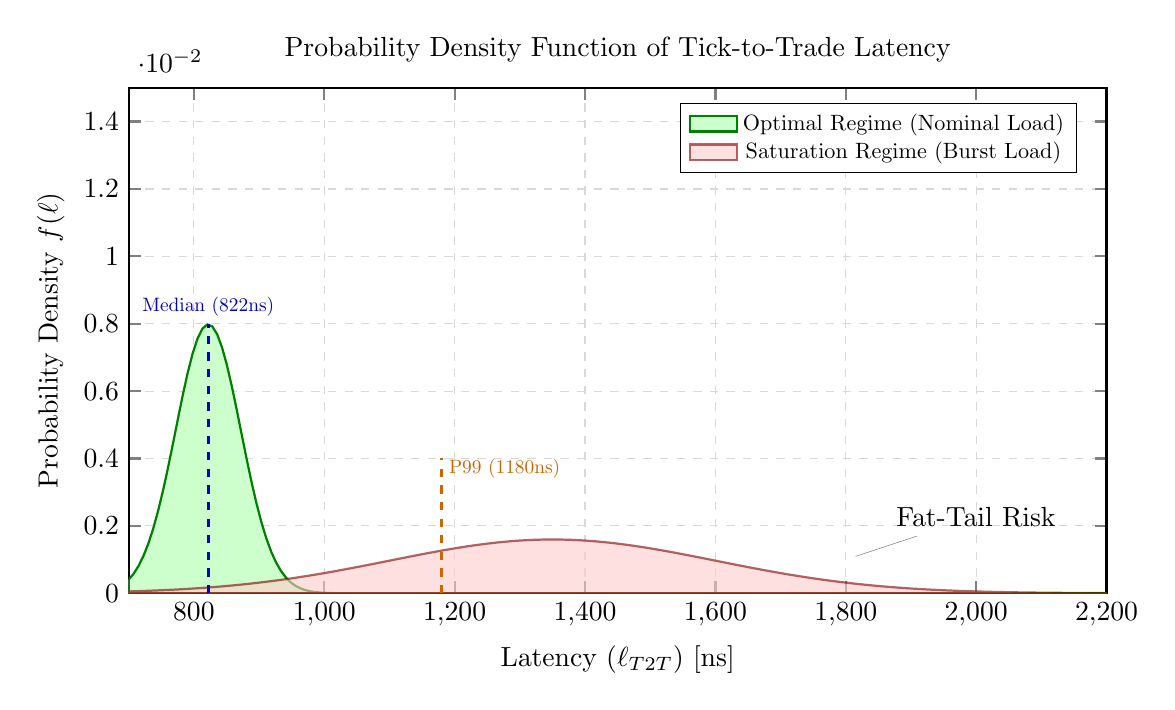
\begin{tikzpicture}
\begin{axis}[
    width=14cm,
    height=8cm,
    xlabel={Latency ($\ell_{T2T}$) [ns]},
    ylabel={Probability Density $f(\ell)$},
    grid=major,
    grid style={dashed, gray!30},
    xmin=700, xmax=2200,
    ymin=0, ymax=0.015,
    title={Probability Density Function of Tick-to-Trade Latency},
    legend pos=north east,
    legend style={nodes={scale=0.8, transform shape}},
    samples=200,
    domain=700:2200,
    axis line style={thick},
    tick style={thick}
]

% PDF definition using a Log-Normal like approach but for visualization we use a shifted Gaussian-like tail
% f(x; mu, sigma) = (1/(x*sigma*sqrt(2pi))) * exp(-(lnx - mu)^2 / 2sigma^2)
% Since pgfplots doesn't have a built-in lognormal PDF, we approximate for visualization 
% with a skewed distribution that looks like typical HFT latency profiles.

% 1. Optimal Regime (Deterministic, low variance)
% mu ~ 820, sigma ~ 40
\addplot [
    fill=green!20,
    draw=green!50!black,
    area legend,
    thick
] { (1/(50 * sqrt(2*pi))) * exp(-( (x - 822)^2 ) / (2 * 50^2)) } \closedcycle;
\addlegendentry{Optimal Regime (Nominal Load)}

% 2. Saturation Regime (Fat tail, higher variance, shifted mean)
% mu ~ 1300, sigma ~ 200
\addplot [
    fill=red!20,
    draw=red!50!black,
    opacity=0.6,
    area legend,
    thick
] { (1/(250 * sqrt(2*pi))) * exp(-( (x - 1350)^2 ) / (2 * 250^2)) } \closedcycle;
\addlegendentry{Saturation Regime (Burst Load)}

% 3. Vertical lines for P50 and P99 (Deterministic Boundaries)
\draw [dashed, blue!80!black, line width=1pt] (axis cs:822, 0) -- (axis cs:822, 0.008) 
    node[above, scale=0.7, pos=1.0] {Median (822ns)};

\draw [dashed, orange!80!black, line width=1pt] (axis cs:1180, 0) -- (axis cs:1180, 0.004) 
    node[above right, scale=0.7, pos=0.8] {P99 (1180ns)};

% Annotations
\node[pin=30:{Fat-Tail Risk}] at (axis cs:1800, 0.001) {};

\end{axis}
\end{tikzpicture}
}
\end{center}
